\documentclass[convert={density=600,size=1080x800,outext=.png}]{standalone}

\usepackage{tikz}
\usetikzlibrary{calc}

\begin{document}
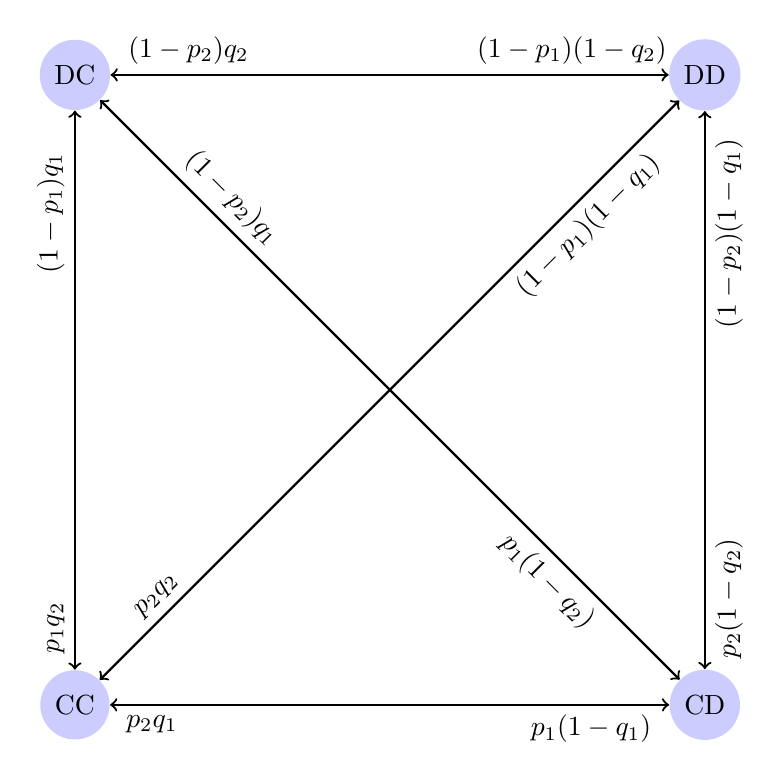
\begin{tikzpicture}
    \node (CC) at (0,0) [circle, fill=blue!20] {CC};
    \node (CD) at ($(CC) + (8, 0)$) [circle, fill=blue!20] {CD};
    \node (DC) at ($(CC) + (0, 8)$) [circle, fill=blue!20] {DC};
    \node (DD) at ($(CC) + (8, 8)$) [circle, fill=blue!20] {DD};

    \draw (CC) edge[out=0, in=180, <->, thick]
            node [below right, near end] {$p_1(1-q_1)$}
            node [below left, very near start] {$p_2q_1$} (CD);

    \draw (CC) edge[out=90, in=-90, <->, thick]
            node [above left, pos=.95, sloped] {$(1 - p_1)q_1$}
            node [above left, very near start, sloped] {$p_1q_2$} (DC);

    \draw (CC) edge[out=45, in=-135, <->, thick]
            node [below right, pos=.7, sloped] {$(1-p_1)(1-q_1)$}
            node [above left, pos=.15, sloped] {$p_2q_2$} (DD);

    \draw (CD) edge[out=135, in=-45, <->, thick]
        node [above right, pos=.9, sloped] {$(1-p_2)q_1$}
        node [below left, pos=.1, sloped] {$p_1(1-q_2)$} (DC);

    \draw (CD) edge[out=90, in=-90, <->, thick]
        node [below right, pos=.6, sloped] {$(1-p_2)(1-q_1)$}
        node [below right, pos=0, sloped] {$p_2(1-q_2)$} (DD);

    \draw (DC) edge[out=0, in=180, <->, thick]
        node [above right, pos=.65] {$(1-p_1)(1-q_2)$}
        node [above left, near start] {$(1-p_2)q_2$} (DD);
\end{tikzpicture}
\end{document}
